\documentclass{ximera}

\graphicspath{{./content/02_2_velocity_and_speed/graphics/}{./graphics/}}

\title{Velocity, Speed, and Acceleration}
\author{Melissa Lynn}
\outcome{Understand the definitions and geometric significance of velocity, speed, and acceleration of a parametric curves, and be able to compute them.}

\begin{document}
\begin{abstract}
\end{abstract}
\maketitle


Consider a path $\vec{x}:I\subset\mathbb{R}\rightarrow\mathbb{R}^n$ which parametrizes a curve in $\mathbb{R}^n$. We often think about this as a particle tracing out the curve as time, given by $t$, passes. We would like to be able to understand and describe the motion of the particle on the curve, and find its velocity and speed, in particular. In order to do this, we need to figure out how to differentiate a path.

Before we define the derivative of a path, we quickly review the single variable definition of a derivative, given in Calculus I.

Given a single variable function $f(x)$, we found the instantaneous rate of change at $x$ of this function by taking the derivative of $f$ at $x$. The derivative also told us the slope of the tangent line at $x$. In order to compute this, we imagined finding the slope of secant lines getting closer and closer to the point. Taking a limit, we obtained the slope of the tangent line.

\begin{image}
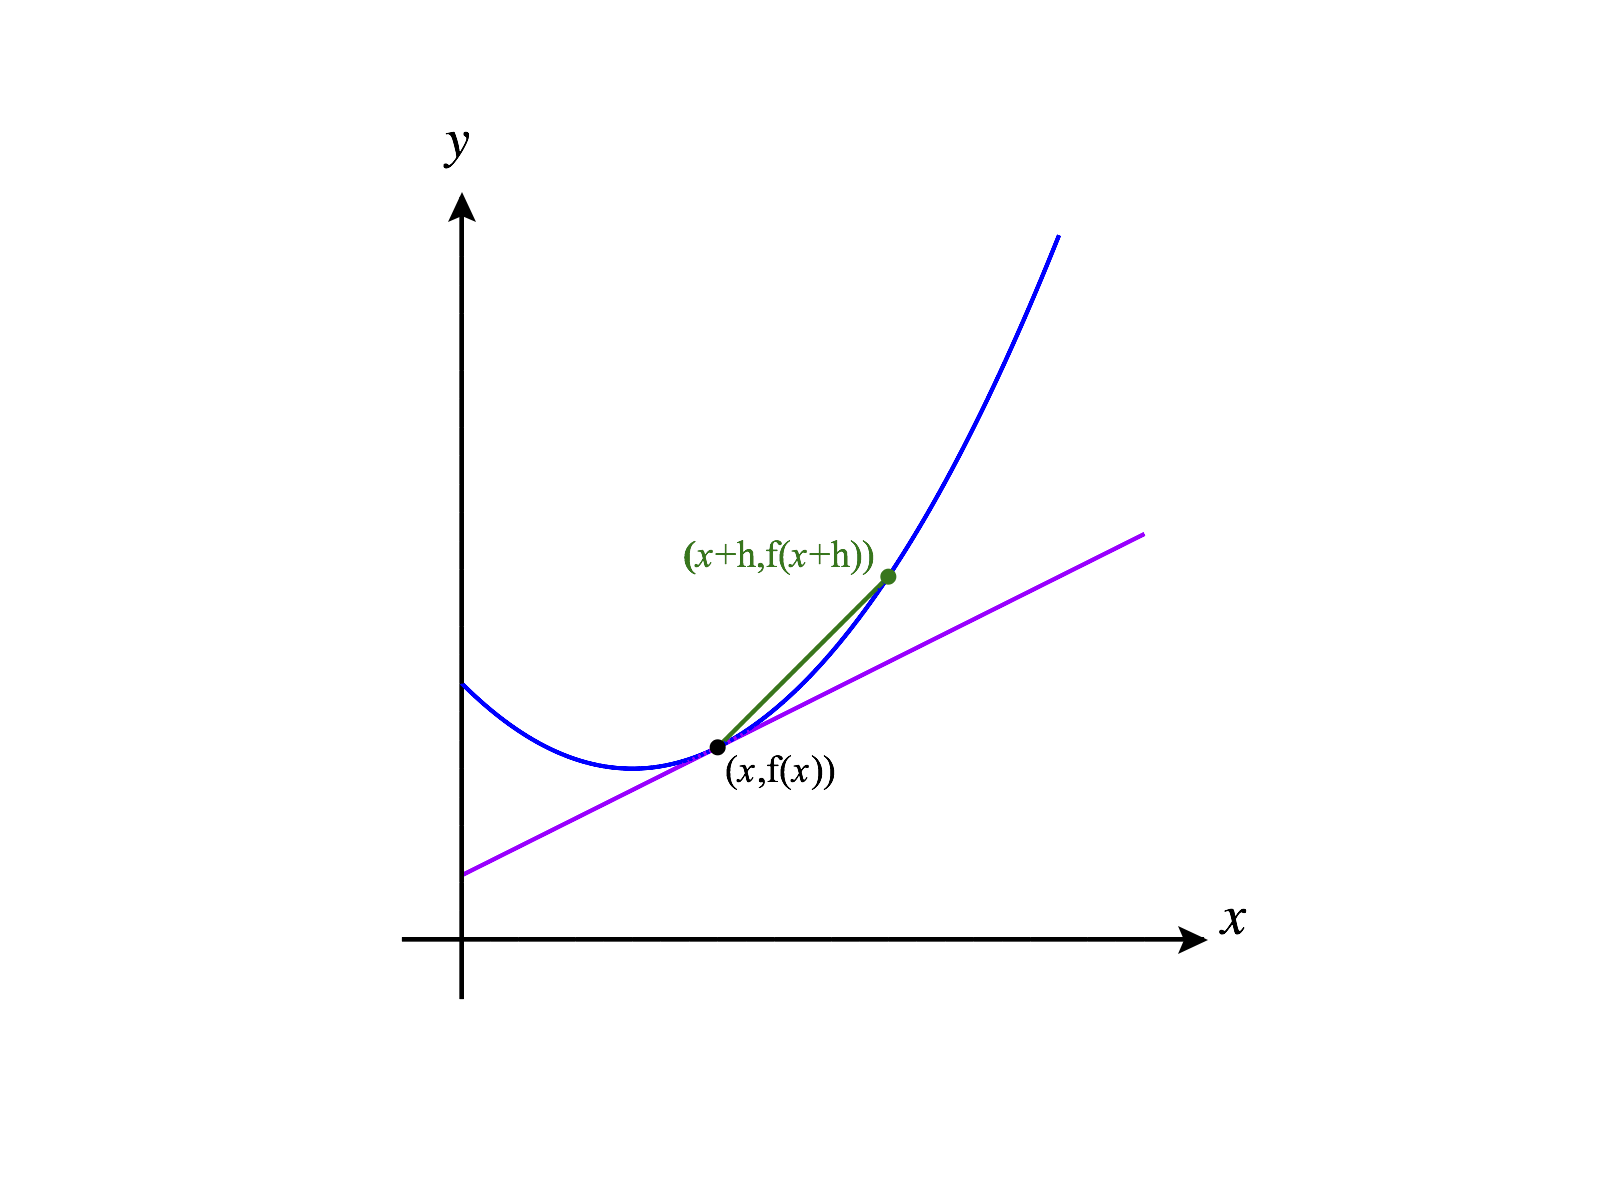
\includegraphics[width=\textwidth]{CalcPlot3D-sv_deriv}
\end{image}

The slope of the secant line through the points $(x,f(x))$ and $(x+h,f(x+h))$ is given by $\dfrac{f(x+h)-f(x)}{h}$, so we defined the derivative of $f$ at $x$ to be
\[
f'(x) = \lim_{h\rightarrow 0}\frac{f(x+h)-f(x)}{h}.
\]

\section*{Derivatives}

We use the same idea for a path $\vec{x}$ in $\mathbb{R}^n$. We consider secant vectors from $\vec{x}(t)$ to $\vec{x}(t+h)$ as $h\rightarrow 0$.

\begin{image}
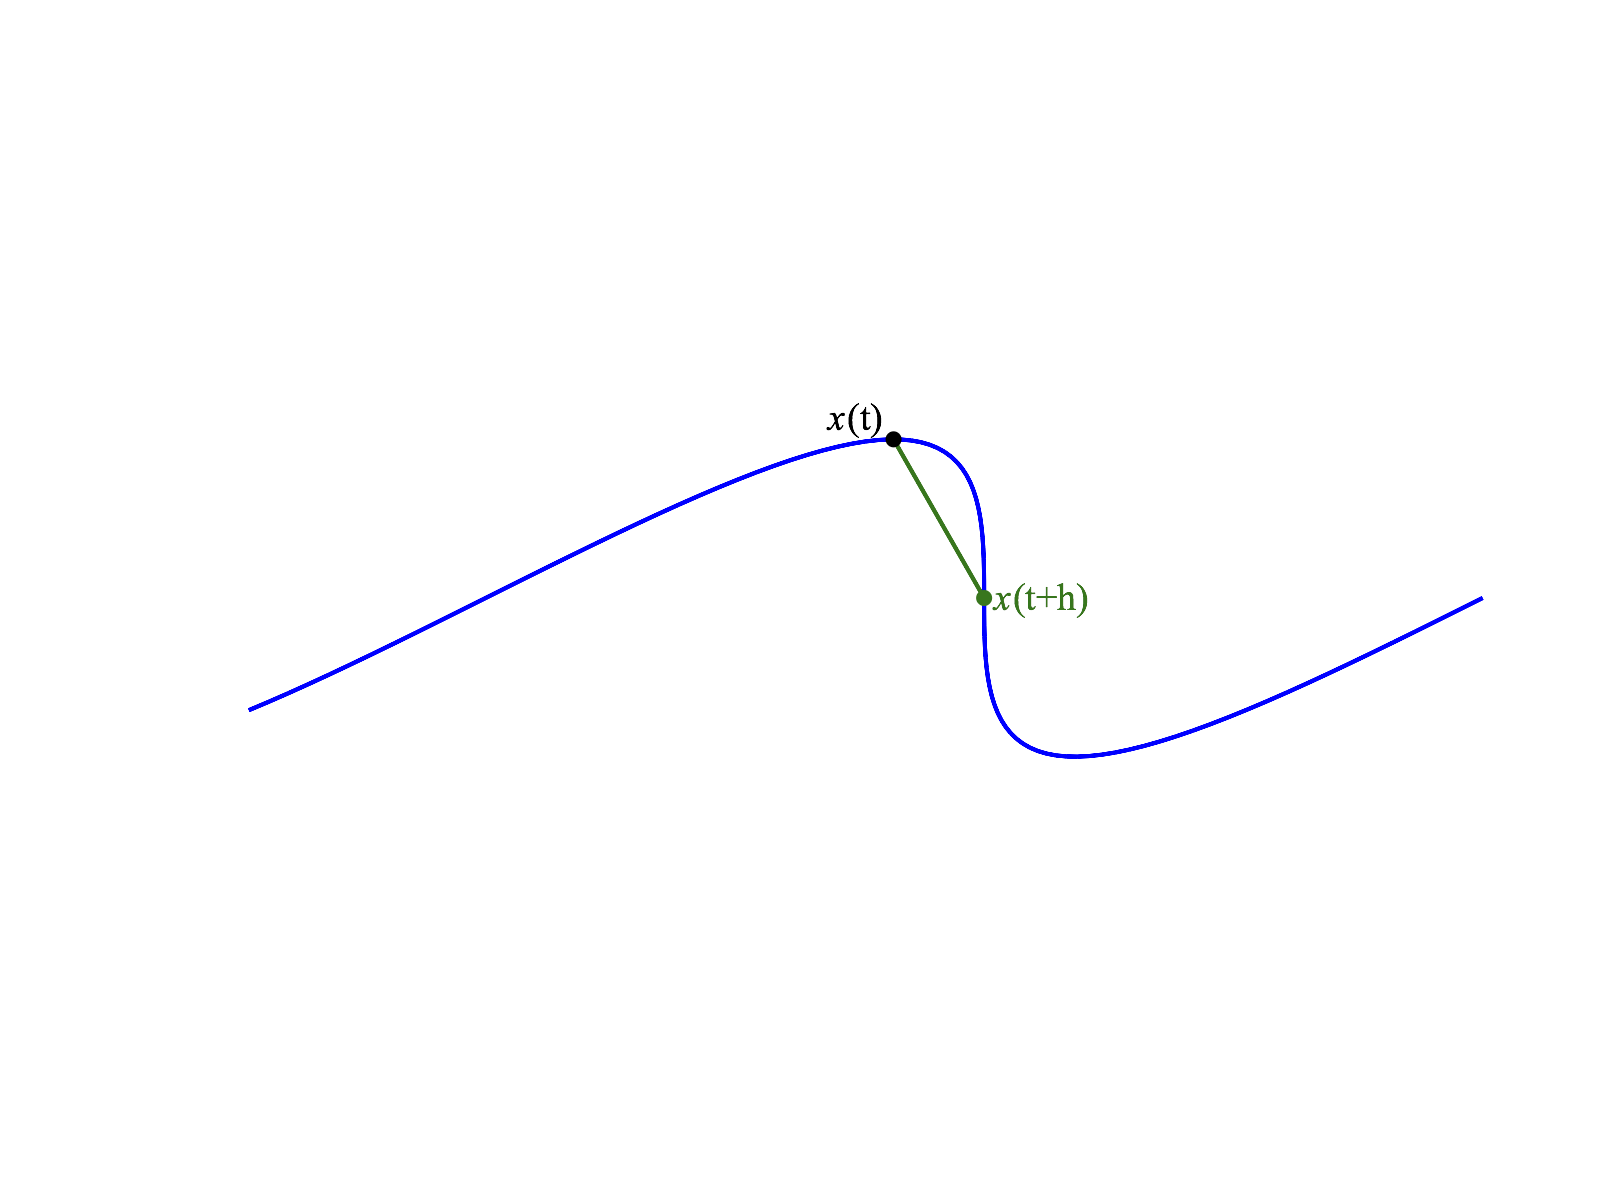
\includegraphics[width=\textwidth]{CalcPlot3D-curve_deriv}
\end{image}

To define the derivative, we will scale these vectors to account for the change in the parameter and then take a limit.

Later, we will see that limits for multivariable functions are difficult to define and compute in general. Fortunately, for paths, limits are fairly simple: we just take the limit of the components. We now define limits along paths, along with continuous paths.

\begin{definition}
Let $\vec{x}:I\rightarrow\mathbb{R}^n$ be a path in $\mathbb{R}^n$, defined on an interval $[a,b]$. Let $x_1,...,x_n$ be the component functions of $\vec{x}$, so that $\vec{x}(t)=(x_1(t),...,x_n(t))$. For $t_0\in (a,b)$, we define the \emph{limit} of $\vec{x}$ as $t$ approaches $t_0$ to be
\[
\lim_{t\rightarrow t_0}\vec{x}(t) = \left(\lim_{t\rightarrow t_0}x_1(t),...,\lim_{t\rightarrow t_0}x_n(t)\right).
\]

A path $\vec{x}:I\rightarrow\mathbb{R}^n$ is \emph{continuous} at $t_0\in I$ if $\lim_{t\rightarrow t_0}\vec{x}(t) = \vec{x}(t_0)$.
\end{definition}

Now that we've defined limits of paths, we are ready to define the derivative of a path as a limit of secant vectors.

\begin{definition}
Let $\vec{x}:I\subset\mathbb{R}\rightarrow\mathbb{R}^n$ be a path in $\mathbb{R}^n$. We define the derivative of $\vec{x}$ at $t$ to be
\[
\vec{x}'(t) = \lim_{h\rightarrow 0} \frac{\vec{x}(t+h) - \vec{x}(t)}{h},
\]
if the limit exists.

We also call $\vec{x}'(t)$ the \emph{velocity vector} of $\vec{x}$, and denote it as $\vec{v}(t)$.
\end{definition}

We'll often draw the velocity vector starting at the give point, and we can then see how it's tangent to the curve.

\begin{image}
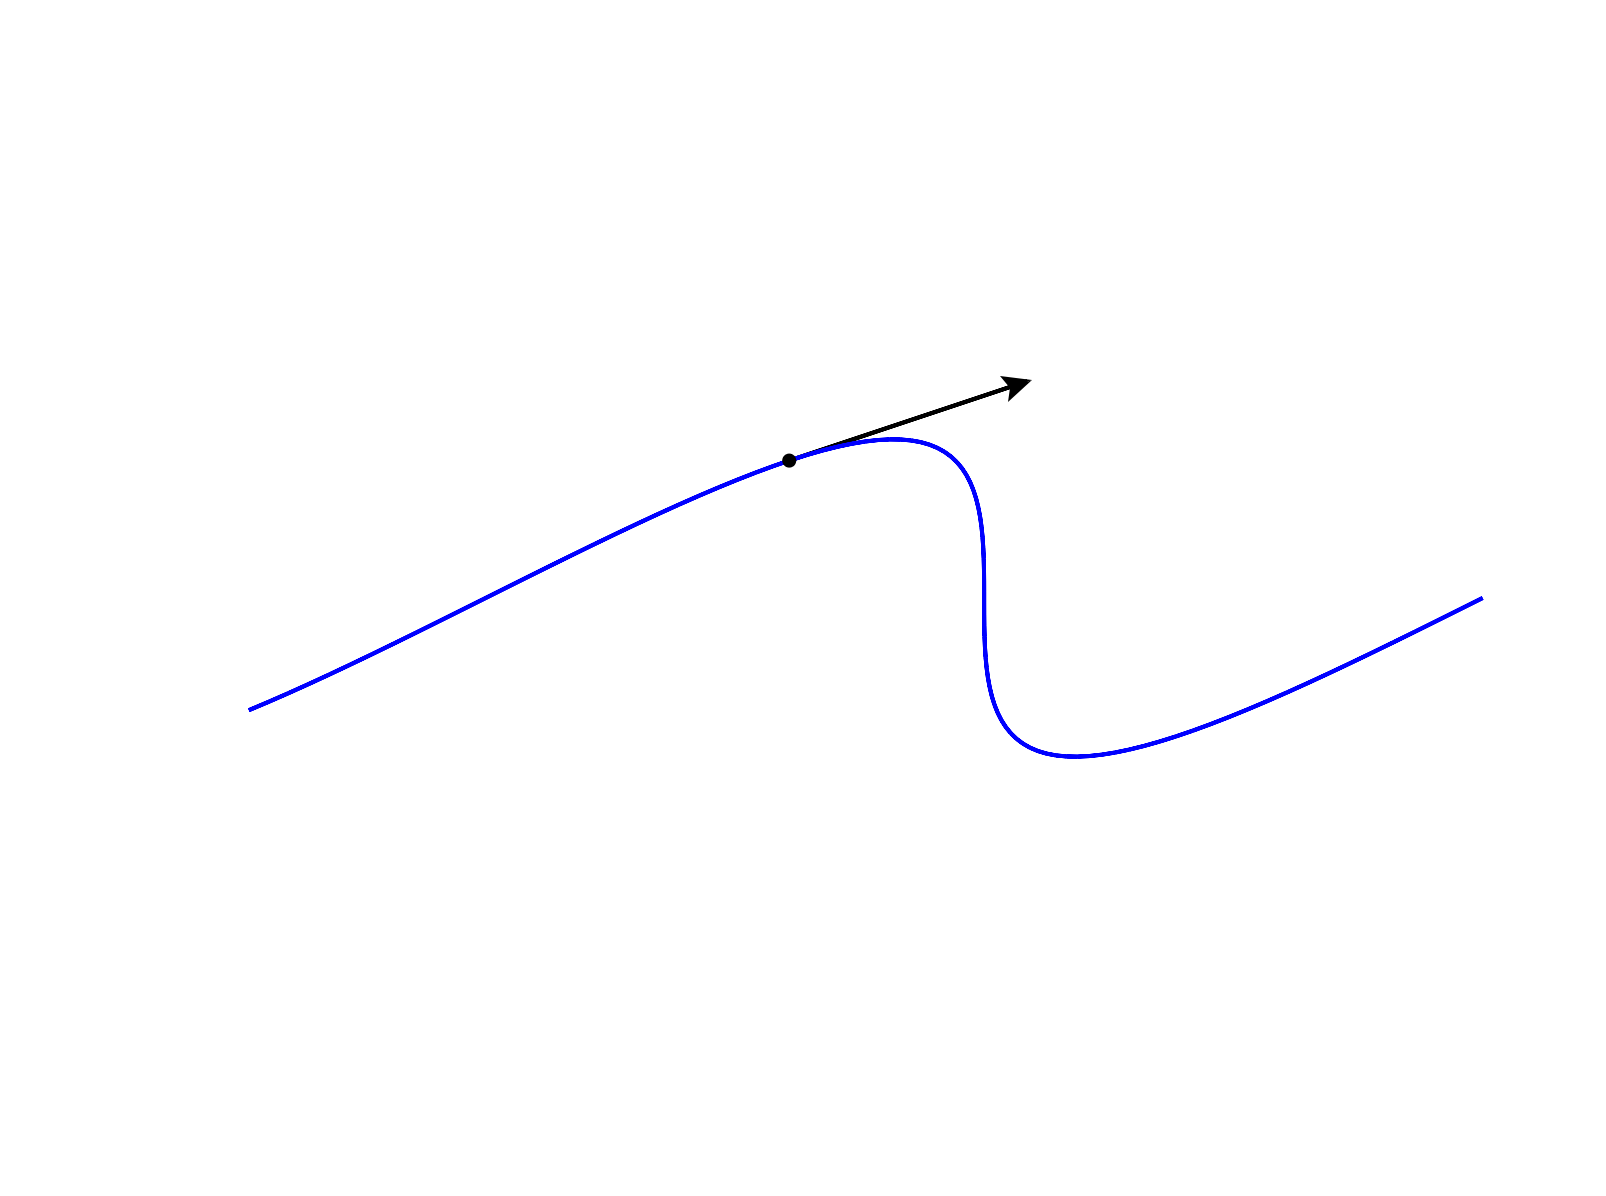
\includegraphics[width=\textwidth]{CalcPlot3D-vel_vector}
\end{image}

We can also see how the velocity vector changes as we move along a curve.

\youtube{waxAKBuX4Fc}

When we first defined derivatives in Calculus I, we spent weeks figuring out how to compute them. We started computing using only the limit definition, then we introduced the power rule, the product rule, the chain rule, and so on. Fortunately, we don't need to repeat this process in Multivariable Calculus: we can take advantage of our previous experience computing derivatives. In order to see why this is the case, let's take another look at our definition for the derivative of a path.

We have $\vec{x}'(t) = \lim_{h\rightarrow 0} \frac{\vec{x}(t+h) - \vec{x}(t)}{h}$ for a path $\vec{x}$. We can write out the path $\vec{x}$ in terms of its components, so
\[
\vec{x}(t) = (x_1(t),...,x_n(t)).
\]
Substituting this into the limit, we have
\begin{align*}
\vec{x}'(t) &= \lim_{h\rightarrow 0} \frac{\vec{x}(t+h) - \vec{x}(t)}{h},\\
&= \lim_{h\rightarrow 0}\frac{(x_1(t+h),...,x_n(t+h)) - (x_1(t),...,x_n(t))}{h},\\
&= \lim_{h\rightarrow 0}\frac{(x_1(t+h) - x_1(t),...,x_n(t+h) - x_1(t))}{h}.
\end{align*}
Dividing through by the scalar $h$ and bringing the limit inside of the vector, we have 
\begin{align*}
\vec{x}'(t) &= \lim_{h\rightarrow 0}\left(\frac{x_1(t+h) - x_1(t)}{h},...,\frac{x_n(t+h) - x_1(t)}{h}\right),\\
&= \left(\lim_{h\rightarrow 0}\frac{x_1(t+h) - x_1(t)}{h},...,\lim_{h\rightarrow 0}\frac{x_n(t+h) - x_1(t)}{h}\right).
\end{align*}

Looking at the limits inside of the components, they should look familiar. They're derivatives of single variable functions! That is, we now have 
\[
\vec{x}'(t) = (x_1'(t),...,x_n'(t)).
\]
This means that we can differentiate a path by differentiating its components, thus taking advantage of our knowledge of single variable derivatives.

\begin{proposition}
We can differentiate a path by differentiating its components. That is,
\[
\vec{x}'(t) = (x_1'(t),...,x_n'(t)).
\]
\end{proposition}

\begin{example}
Consider the path $\vec{x}(t) = (\cos(t), \sin(t))$ for $0\leq t\leq 2\pi$, which parametrizes the unit circle in $\mathbb{R}^2$. We compute the derivative of this path,
\begin{align*}
\vec{x}'(t) &= \left(\frac{d}{dt}\cos(t), \frac{d}{dt}\sin(t)\right)\\
&= \left(-\sin(t), \cos(t)\right).
\end{align*}

We can see how the velocity vector changes as $t$ increases from $0$ to $2\pi$. Notice that it's always tangent to the circle.

\youtube{MojL8LAKTso}

\end{example}

\begin{problem}
Consider the path $\vec{y}(t) = (t^2,t^3)$ for $0\leq t\leq 1$. Compute the velocity vector.
\[
y'(t) = \answer{(2t, 3t^2)}
\]

Consider the path $\vec{z}(t) = \left(t, e^{t^2}\right)$ for $-\infty < t < \infty$. Compute the velocity vector.
\[
z'(t) = \answer{(1, 2te^{t^2})}
\]
\end{problem}

\begin{example}
We can similarly compute the velocity of a path in $\mathbb{R}^3$, or $\mathbb{R}^n$ for any $n$. Let's compute the velocity of the ``tornado,''
\[
\vec{x}(t) = (t\cos(t),t\sin(t),t),
\]
for $t\in [0,20]$. Remembering to use the product rule, we have
\[
\vec{x}'(t) = \answer{(\cos(t)-t\sin(t),\sin(t)+t\cos(t), 1)}.
\]
We can see how the velocity vector changes as $t$ increases from $0$ to $20$.

\youtube{dVoY9sHH2g4}
\end{example}

\section*{Speed}

We defined the derivative $\vec{x}'$ of a path $\vec{x}$, thinking of a limit of scaled secant vectors. Taking the limit of these vectors, our derivative gives us a vector which is tangent to the path.

\begin{image}
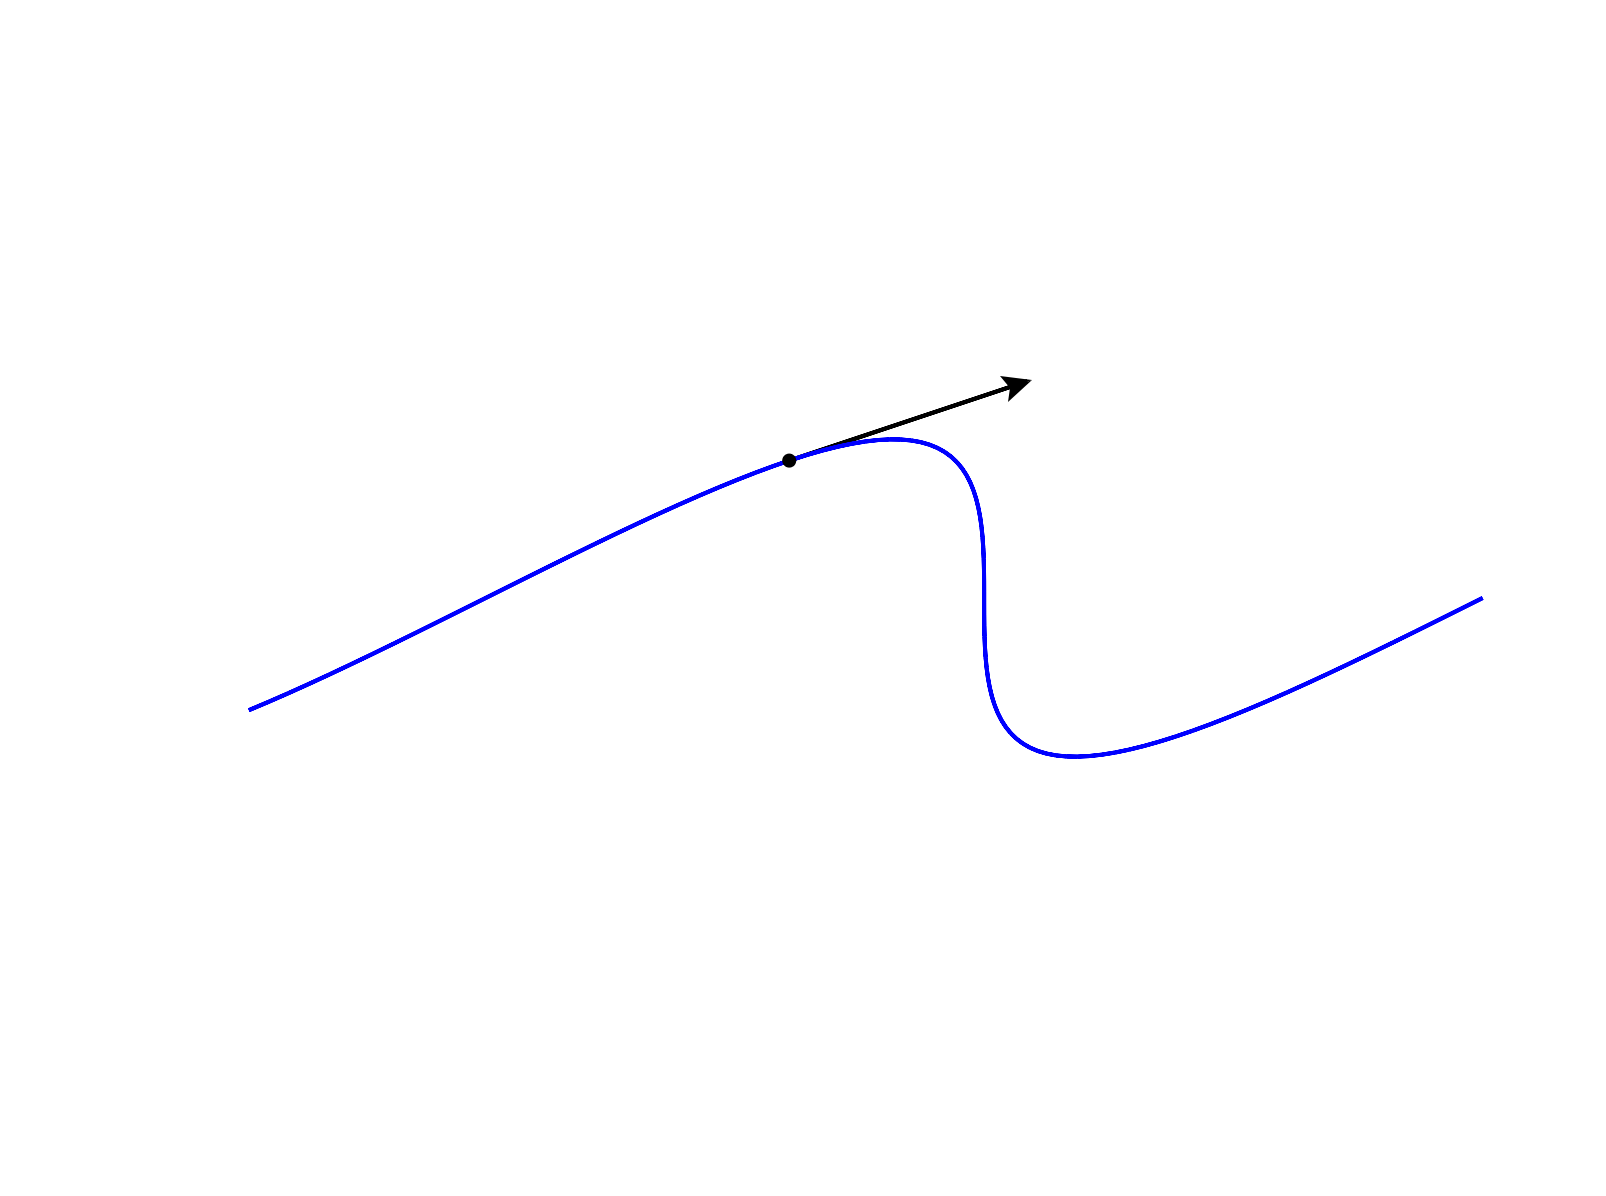
\includegraphics[width=\textwidth]{CalcPlot3D-vel_vector}
\end{image}

The direction of $\vec{x}'$ gives us the direction of instantaneous of a particle moving along the path, and the length of $\vec{x}'$ tells us the speed of the particle. Recall that we sometimes refer to $\vec{x}'$ as the velocity vector, and write it as $\vec{v}$.

\begin{definition}
Consider a path $\vec{x}:I\subset\mathbb{R}\rightarrow\mathbb{R}^n$.

We previously defined the velocity vector of $\vec{x}$ at $t$ to be $\vec{v}(t) = \vec{x}'(t)$. The velocity vector is tangent to $\vec{x}$ at $\vec{x}(t)$.

The \emph{speed} of $\vec{x}$ at $t$ is $\|\vec{x}'(t)\| = \|\vec{v}(t)\|$.
\end{definition}

\begin{example}
Consider the path $\vec{x}(t) = (\cos(t), \sin(t))$ for $0\leq t \leq 2\pi$, which parametrizes the unit circle in $\mathbb{R}^2$. We previously computed the velocity of this path as
\[
\vec{v}(t) = \vec{x}'(t) = (-\sin(t), \cos(t)).
\]
We can then compute the speed of $\vec{x}$ as
\begin{align*}
\|\vec{x}'(t)\| &= \|(-\sin(t), \cos(t))\|,\\
&= \sqrt{(-\sin(t))^2 + (\cos(t))^2},\\
& = \sqrt{1},\\
& = 1.
\end{align*}

Consider the path $\vec{y}(t) = (\cos(t^2), \sin(t^2))$ for $0\leq t\leq \sqrt{2\pi}$. This also parametrizes the unit circle in $\mathbb{R}^2$. The velocity vector of this path is
\[
\vec{y}'(t) = \answer{(-2t\sin(t^2), 2t\cos(t^2))}.
\]
The speed of this path is
\[
\|\vec{y}'(t)\| = \answer{2t}.
\]

Although both of these paths parametrize the unit circle counterclockwise and starting and ending at $(1,0)$, they do so in different ways. The first path, $\vec{x}$, traverses the unit circle at constant speed. The second path, $\vec{y}$, travels very slowly at first, then the speed increases as it travels around the circle.
\end{example}

\begin{example}
Consider the path $\vec{x}(t)=(\cos(t),\sin(t),t)$ in $\mathbb{R}^3$. The velocity vector of this path is
\[
\vec{v}(t) = \answer{(-\sin(t),\cos(t),1)},
\]
And the speed of this path is
\[
\|\vec{v}(t)\| = \answer{\sqrt{2}}.
\]
\end{example}

\section*{Acceleration}

Given a path $\vec{x}(t)$ in $\mathbb{R}^n$ defined on an interval $I$, we've seen that we can compute it's velocity, $\vec{v}(t) = \vec{x}'(t)$. We can view the velocity as a function from $I$ to $\mathbb{R}^n$, which gives us another path in $\mathbb{R}^n$. We can then differentiate $\vec{v}(t)$, giving us a sort of ``second derivative'' of our original path $\vec{x}(t)$. We call this the \emph{acceleration} of $\vec{x}(t)$, and denote it by $\vec{x}''(t)$ or $\vec{a}(t)$.

\begin{example}
We'll compute the acceleration of the path $\vec{x}(t) = (t,t^2,t^3)$ in $\mathbb{R}^3$.

First, we compute the velocity, by differentiating the given path.
\[
\vec{x}'(t) = \answer{(1,2t,3t^3)}
\]
Then, we differentiate again, to find the acceleration.
\[
\vec{x}''(t) = \answer{(0,2,9t)}
\]
\end{example}

As you can imagine, we could continue to take higher and higher derivatives of our path. In most cases, the velocity and acceleration will provide the most useful information about the path, so we'll typically stop there. However, some theorems will have requirements about differentiability, so we'll classify functions based on how differentiable they are.

\begin{definition}
Let $\vec{x}:I\rightarrow\mathbb{R}^n$ be a path in $\mathbb{R}^n$. We say that $\vec{x}(t)$ is \emph{of class} $C^k$ if the $k$th derivative of $\vec{x}(t)$ exists and is continuous.

If $\vec{x}(t)$ has continuous derivatives of all orders, then we say that $\vec{x}(t)$ is \emph{of class} $C^{\infty}$. In this case, we also say that $\vec{x}(t)$ is \emph{smooth}.
\end{definition}


\section*{Parametrizing the tangent line}

Consider a path $\vec{x}:I\subset\mathbb{R}\rightarrow\mathbb{R}^n$. The velocity of this path gives us a vector $\vec{x}'(t)$ tangent to the curve at $\vec{x}(t)$. The tangent line to $\vec{x}$ at $\vec{x}(t)$ passes through the point $\vec{x}(t)$ and is parallel to the vector $\vec{x}'(t)$. This allows us to parametrize the tangent line, however we need to be very careful to distinguish between the parameter for the \emph{line} and the parameter for the \emph{path}. We do this by taking the parameter for our curve to be $t_0$ at our chosen point, so we are working with the point $\vec{x}(t_0)$ and the tangent vector $\vec{x}'(t_0)$.

\begin{proposition}
Consider a path $\vec{x}:I\subset\mathbb{R}\rightarrow\mathbb{R}^n$. We can parametrize the line tangent to $\vec{x}$ at $\vec{x}(t_0)$ as
\[
\vec{l}(t) = \vec{x}(t_0) + t\vec{x}'(t_0) \textrm{ for } -\infty < t < \infty.
\]
\end{proposition}

Note that it's particularly important to allow the parameter $t$ to be any real number, otherwise we will be missing part of the line.

\begin{example}
As an example, we'll find a parametrization for the tangent line to the path $\vec{x}(t)=(\cos(t),\sin(t),t)$, when $t=0$. The derivative is
\[
\vec{x}'(t) = \answer{(-\sin(t),\cos(t),1)}.
\]
When $t=0$, this is
\[
\vec{x}'(0) = \answer{(0,1,1)}.
\]
When $t=0$, we have
\[
\vec{x}(0) = \answer{(1,0,0)}.
\]
Parametrizing the tangent line, we have
\begin{align*}
\vec{l}(t) &= \vec{x}(0) + t\vec{x}'(0)\\
&= \answer{(1,t,t)},
\end{align*}
for $-\infty < t < \infty$.

Below, we have the graph of the curve parametrized by $\vec{x}(t)$, along with its tangent line when $t=0$.

\begin{image}
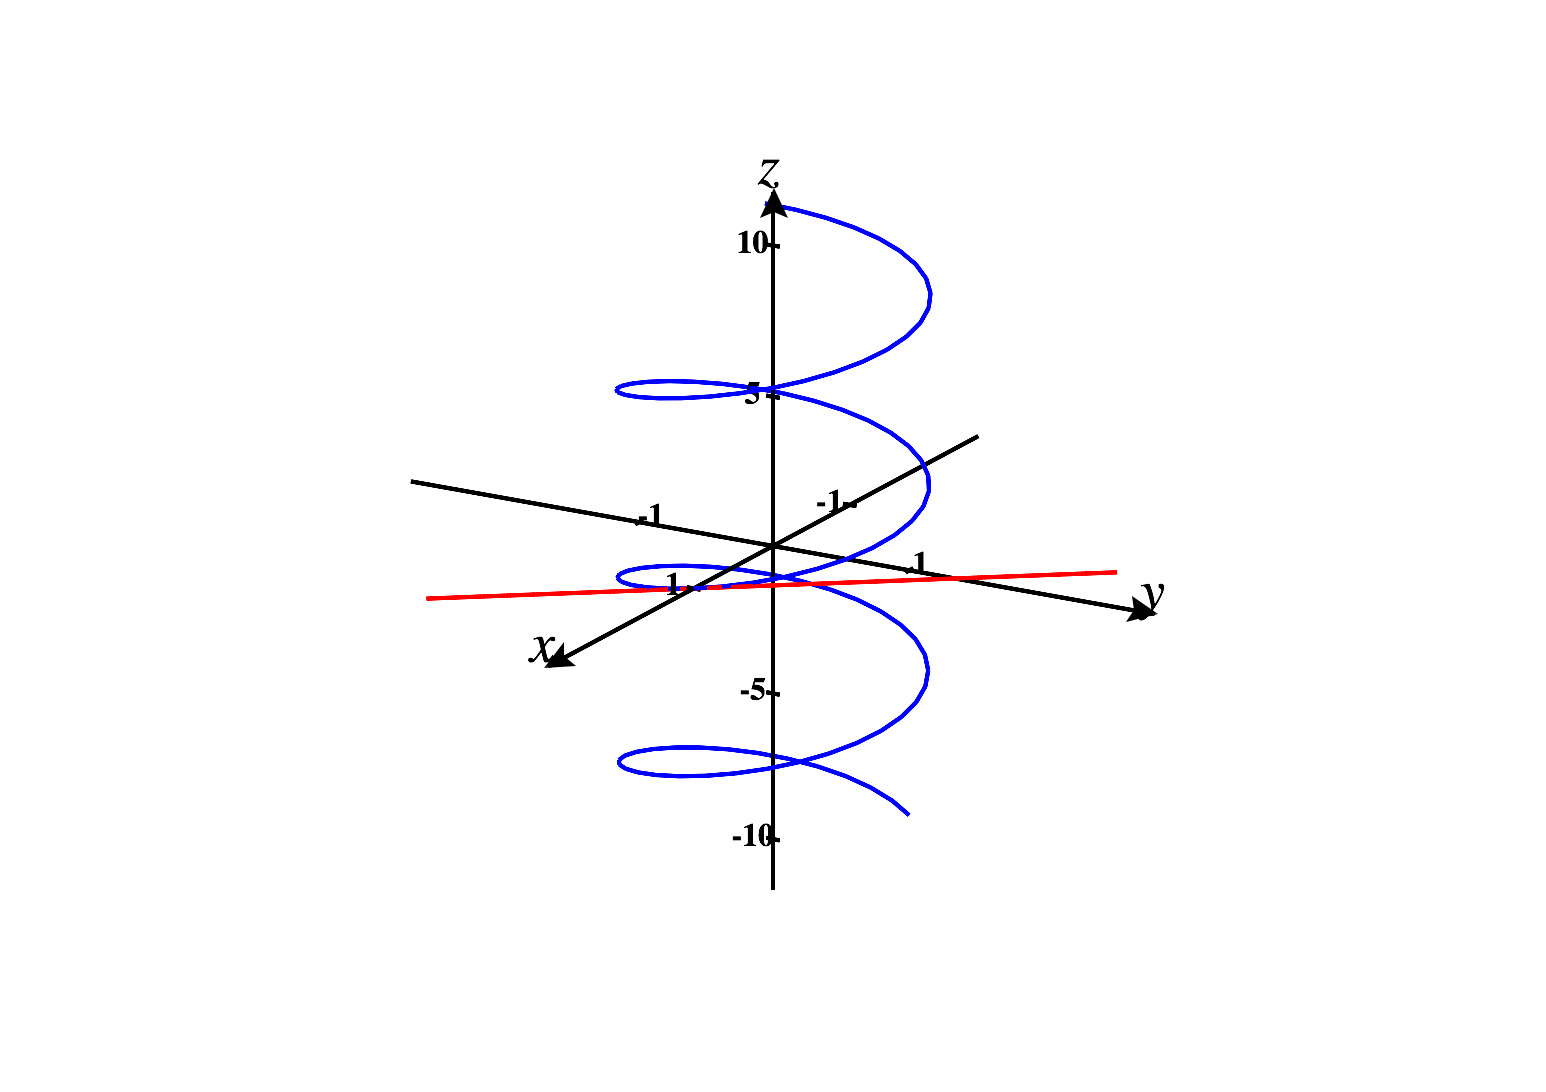
\includegraphics[width=\textwidth]{CalcPlot3D-tangent_line}
\end{image}
\end{example}

\textit{Images were generated using \href{https://www.monroecc.edu/faculty/paulseeburger/calcnsf/CalcPlot3D/}{CalcPlot3D}.}


\end{document}